% Use this template to write your solutions to COS 423 problem sets

\documentclass[12pt]{article}
\usepackage[utf8]{inputenc}
\usepackage{amsmath, amsfonts, amsthm, amssymb, algorithm, graphicx, mathtools, xfrac}
\usepackage[noend]{algpseudocode}
\usepackage{fancyhdr, lastpage}
\usepackage{booktabs}
\usepackage{multirow}
\usepackage{graphicx}
\usepackage{pgfplots}
\usepackage[vmargin=1.20in,hmargin=1.25in,centering,letterpaper]{geometry}
\setlength{\headsep}{.50in}
\setlength{\headheight}{15pt}

% Landau notation
\DeclareMathOperator{\BigOm}{\mathcal{O}}
\newcommand{\BigOh}[1]{\BigOm\left({#1}\right)}
\DeclareMathOperator{\BigTm}{\Theta}
\newcommand{\BigTheta}[1]{\BigTm\left({#1}\right)}
\DeclareMathOperator{\BigWm}{\Omega}
\newcommand{\BigOmega}[1]{\BigWm\left({#1}\right)}
\DeclareMathOperator{\LittleOm}{\mathrm{o}}
\newcommand{\LittleOh}[1]{\LittleOm\left({#1}\right)}
\DeclareMathOperator{\LittleWm}{\omega}
\newcommand{\LittleOmega}[1]{\LittleWm\left({#1}\right)}

% argmin and argmax
\newcommand{\argmin}{\operatornamewithlimits{argmin}}
\newcommand{\argmax}{\operatornamewithlimits{argmax}}

\newcommand{\calP}{\mathcal{P}}
\newcommand{\Z}{\mathbb{Z}}
\newcommand{\R}{\mathbb{R}}
\newcommand{\Exp}{\mathbb{E}}
\newcommand{\Q}{\mathbb{Q}}
\newcommand{\sign}{\mathrm{sign\ }}
\newcommand{\abs}{\mathrm{abs\ }}
\newcommand{\eps}{\varepsilon}
\newcommand{\zo}{\{0, 1\}}
\newcommand{\SAT}{\mathit{SAT}}
\renewcommand{\P}{\mathbf{P}}
\newcommand{\NP}{\mathbf{NP}}
\newcommand{\coNP}{\co{NP}}
\newcommand{\co}[1]{\mathbf{co#1}}
\renewcommand{\Pr}{\mathop{\mathrm{Pr}}}

% theorems, lemmas, invariants, etc.
\newtheorem{theorem}{Theorem}
\newtheorem{lemma}[theorem]{Lemma}
\newtheorem{invariant}[theorem]{Invariant}
\newtheorem{corollary}[theorem]{Corollary}
\newtheorem{definition}[theorem]{Definition}
\newtheorem{property}[theorem]{Property}
\newtheorem{proposition}[theorem]{Proposition}

% piecewise functions
\newenvironment{piecewise}{\left \{\begin{array}{l@{,\ }l}}
{\end{array}\right.}

% paired delimiters
\DeclarePairedDelimiter{\ceil}{\lceil}{\rceil}
\DeclarePairedDelimiter{\floor}{\lfloor}{\rfloor}
\DeclarePairedDelimiter{\len}{|}{|}
\DeclarePairedDelimiter{\set}{\{}{\}}

\makeatletter
\@addtoreset{equation}{section}
\makeatother
\renewcommand{\theequation}{\arabic{section}.\arabic{equation}}

% algorithms
\algnewcommand\algorithmicinput{\textbf{INPUT:}}
\algnewcommand\INPUT{\item[\algorithmicinput]}
\algnewcommand\algorithmicoutput{\textbf{OUTPUT:}}
\algnewcommand\OUTPUT{\item[\algorithmicoutput]}


% Formating Macros

\pagestyle{fancy}
\lhead{\sc \hmwkClass\ $\; \;\cdot \; \;$ \hmwkSemester\ $\; \;\cdot \; \;$
Problem \hmwkAssignmentNum.\hmwkProblemNum}
%\chead{\sc Problem \hmwkAssignmentNum.\hmwkProblemNum}
%\chead{}
\rhead{\em \hmwkAuthorName\ $($\hmwkAuthorID$)$\/}
\cfoot{}
\lfoot{}
\rfoot{\sc Page\ \thepage\ of\ \protect\pageref{LastPage}}
\renewcommand\headrulewidth{0.4pt}
\renewcommand\footrulewidth{0.4pt}

\fancypagestyle{fancycollab}
{
    \lfoot{\textit{Collaborators: \hmwkCollaborators}}
}

\fancypagestyle{problemstatement}
{
    \rhead{}
    \lfoot{}
}

%%%%%% Begin document with header and title %%%%%%%%%%%%%%%%%%%%%%%%%

\begin{document}

%%%%%% Header Information %%%%%%%%%%%%%%%%%%%%%%%%%%%%%%%%%%%%%%%%%%%

%%% Shouldn't need to change these
\newcommand{\hmwkClass}{COS 255}
\newcommand{\hmwkSemester}{Spring 2016}

%%% Your name, in standard First Last format
\newcommand{\hmwkAuthorName}{Lukas Leung}
%%% Your NetID
\newcommand{\hmwkAuthorID}{lleung}

%%% The problem set number (just the number)
\newcommand{\hmwkAssignmentNum}{4}

%%% The problem number (just the number)
\newcommand{\hmwkProblemNum}{0}

%%% A list of your collaborators' NetIDs, separated by ", ".
%%% You can use a new line ("\\") in the middle to prevent a long
%%% list from overflowing.
\newcommand{\hmwkCollaborators}{}
%%% Sets the collaborator list to appear on the first page
\thispagestyle{fancycollab}

%%%%%%% begin Solution %%%%%%%%%%%%%%%%%%%%%%%%%%%%%%%%%%%%%%%%%%%%
%\section{Results from UVA}
%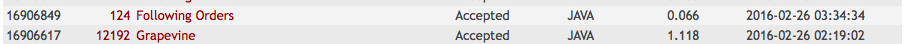
\includegraphics[width=\textwidth]{uvaResults}
%\newpage

%%%%%%% start Problem A %%%%%%%%%%%%%%%%%%%%%%%%%%%%%%%%%%%%%%%%%%%

\section{Problem A: Amalgamated Artichokes}
\textbf{Background} \\
~\indent Explaination...
%%%%%%% end Problem %%%%%%%%%%%%%%%%%%%%%%%%%%%%%%%%%%%%%%%%%%%%%%%

\newpage

%%%%%%% Mathematical Formulation %%%%%%%%%%%%%%%%%%%%%%%%%%%%%%%%%%
\subsection{Mathematical Formulation}
Given an input of integers $p, a, b, c, d, and n$, the formula
$f(x) = p\cdot (sin(a\cdot x + b) + cos(c\cdot x + d) + 2)$ where $x \in [1, n]$, determine the largest
decrease between the integer values $x_i, x_j$ where $i \textless j$ and $x_i \geq x_j$ and there does
not exist another pair $x_k, x_l$ where $k \textless l$ and $x_k \geq x_l$ but $x_k - x_l \textgreater x_i - x_j$.

%%%%%%% Algorithm %%%%%%%%%%%%%%%%%%%%%%%%%%%%%%%%%%%%%%%%%%%%%%%%%

\subsection{Solution}
The main functionality of this algorithm is to plug in each point keeping track of the highest seen point, $h$,
the lowest seen point occuring after $l$, and the largest difference, $d = h-l$. It should be noted that since
we are always taking the difference between the two values, we can factor out the $\cdot p$ as well as neglect
the +2 portions of the formula. Also, to cut down on run time, it works in the java system if you \% pi each of
the entries before putting them into the sine and cosine functions. For whatever reason the larger the input,
the more costly the operation is.

\begin{algorithm}[H]
\caption{Main}
\begin{algorithmic}
    \Procedure{f}{x}
        \State $ab \gets$ (a*x+b) \% pi,
        \State $cd \gets$ (c*x+d) \% pi;
        \State return (Math.sin(ab) + Math.cos(cd))
    \EndProcedure
    \Procedure{Solve}{p, a, b, c, d, n}
        \State $val, h, l \gets$ f(1); $diff \gets$ 0
        \For{x $\in$ [2, n]} // if n = 1, do not execute
            \State $val \gets$ f(x)
            \If{$val \textgreater h$} // higher than current highest
                \State $h, l \gets$ val;
            \ElsIf{$val \textless l$} // lower than current lowest
                \State $l \gets$ val; $curDiff \gets$ h - l;
                \If{$curDiff \textgreater diff$}
                    $diff \gets$ curDiff;
                \EndIf
            \EndIf
        \EndFor
        \State \Call{print}{$p\cdot diff$}
    \EndProcedure
\end{algorithmic}
\end{algorithm}


%%%%%%% Correctness %%%%%%%%%%%%%%%%%%%%%%%%%%%%%%%%%%%%%%%%%%%%%%%

\subsection{Correctness}
%%%%%%% PROPOSITION 1 %%%%%%%%%%%%%%%
\begin{proposition}
~ \\ \indent propose
\end{proposition}

\begin{proof}
~ \\ \indent Using the fact that 
\end{proof}


%%%%%%% Analysis %%%%%%%%%%%%%%%%%%%%%%%%%%%%%%%%%%%%%%%%%%%%%%%%%%
\subsection{Analysis}

%%%%%%% PROPOSITION 1 %%%%%%%%%%%%%%%
\begin{proposition}
\label{numq}
The \underline{space complexity} of this algorithm is \textbf{O(1)}
\end{proposition}

\begin{proof}
~ \\ \indent This is due to the fact that we will only store the values $p, a, b, c, d, n, and diff$
as integer variables O(1):
\begin{center}
    Giving us a space complexity of \textbf{O(1)}
\end{center}
\end{proof}

%%%%%%% PROPOSITION 2 %%%%%%%%%%%%%%%
\begin{proposition}
\label{numq}
The \underline{time complexity} of this algorithm is \textbf{O(N)}
\end{proposition}

\begin{proof}
This is the case because our algorithm goes through the points $1, 2, ..., n$ once and only
calculates each value one time.
\begin{center}
    Giving us a time complexity of \textbf{O(N)}
\end{center}
\end{proof}

%%%%%%% Example %%%%%%%%%%%%%%%%%%%%%%%%%%%%%%%%%%%%%%%%%%%%%%%%%%%

\subsection{An Example}

%%%%%%% end Problem A %%%%%%%%%%%%%%%%%%%%%%%%%%%%%%%%%%%%%%%%%%%%%


%%%%%%% end Solution %%%%%%%%%%%%%%%%%%%%%%%%%%%%%%%%%%%%%%%%%%%%%%

\end{document}